% This is "sig-alternate.tex" V2.0 May 2012
% This file should be compiled with V2.5 of "sig-alternate.cls" May 2012
%
% This example file demonstrates the use of the 'sig-alternate.cls'
% V2.5 LaTeX2e document class file. It is for those submitting
% articles to ACM Conference Proceedings WHO DO NOT WISH TO
% STRICTLY ADHERE TO THE SIGS (PUBS-BOARD-ENDORSED) STYLE.
% The 'sig-alternate.cls' file will produce a similar-looking,
% albeit, 'tighter' paper resulting in, invariably, fewer pages.
%
% ----------------------------------------------------------------------------------------------------------------
% This .tex file (and associated .cls V2.5) produces:
%       1) The Permission Statement
%       2) The Conference (location) Info information
%       3) The Copyright Line with ACM data
%       4) NO page numbers
%
% as against the acm_proc_article-sp.cls file which
% DOES NOT produce 1) thru' 3) above.
%
% Using 'sig-alternate.cls' you have control, however, from within
% the source .tex file, over both the CopyrightYear
% (defaulted to 200X) and the ACM Copyright Data
% (defaulted to X-XXXXX-XX-X/XX/XX).
% e.g.
% \CopyrightYear{2007} will cause 2007 to appear in the copyright line.
% \crdata{0-12345-67-8/90/12} will cause 0-12345-67-8/90/12 to appear in the copyright line.
%
% ---------------------------------------------------------------------------------------------------------------
% This .tex source is an example which *does* use
% the .bib file (from which the .bbl file % is produced).
% REMEMBER HOWEVER: After having produced the .bbl file,
% and prior to final submission, you *NEED* to 'insert'
% your .bbl file into your source .tex file so as to provide
% ONE 'self-contained' source file.
%
% ================= IF YOU HAVE QUESTIONS =======================
% Questions regarding the SIGS styles, SIGS policies and
% procedures, Conferences etc. should be sent to
% Adrienne Griscti (griscti@acm.org)
%
% Technical questions _only_ to
% Gerald Murray (murray@hq.acm.org)
% ===============================================================
%
% For tracking purposes - this is V2.0 - May 2012

\documentclass{sig-alternate}

\usepackage{todonotes,stmaryrd}
\usepackage{cite}
\usepackage{tabularx}
\usepackage{xspace}
\let\endproof\relax
\let\proof\relax
\usepackage{amssymb,amsmath,mathtools,amsthm}
\usepackage{url}
\usepackage{algorithm}
\usepackage[noend]{algorithmic}
\usepackage{float}
\usepackage{subfigure}

\usepackage{enumitem}
\usepackage{multirow}

\newcommand\fakenewspaper[0]{fakenewspaperpl\xspace}

\newcommand\rro[1]{\textbf{#1}.}% \subsection*{#1}}

\usepackage{pifont}


\graphicspath

\newtheorem{theorem}{Theorem}

%\renewcommand{\floatpagefraction}{0.8}% Magic command ! Avoid to have a page with only one figure


%%%%%%%%%%%%%%%%%%%%%%%%%%%%%%%%%%%%%%%%%%%
%%%%%%%% COMMENTS / ANNOTATIONS / TODOS
\newif\ifdraft\drafttrue
% \newif\ifdraft\draftfalse

\ifdraft
\newcommand\todos[1]{\todo[inline]{TODO (all): #1}}
\newcommand\ma[1]{\todo[color=green!40,inline]{TODO (Mathieu): #1}}
\newcommand{\machanged}[1]}
\newcommand\gb[1]{\todo[color=yellow!40,inline]{TODO (Guillaume): #1}}
\newcommand\rb[1]{\todo[color=blue!35,inline, caption={}]{TODO (Razieh): #1}}
\newcommand{\rbc}[1]}
\else
\newcommand\todos[1]{}
\newcommand\ma[1]{}
\newcommand\machanged[1]{#1}
\newcommand\gb[1]{}
\newcommand\rb[1]{}
\newcommand\rbc[1]{#1}
\fi
%%%%%%%%%%%%%%%%%%%%%%%%%%%%%%%%%%%%%%%%%%%

\newcommand{\ie}{\emph{i.e.,}\xspace}
\newcommand{\eg}{\emph{e.g.,}\xspace}
\newcommand{\cf}{\emph{cf.}}
\newcommand{\etal}{\emph{et al.}\xspace}
\newcommand{\etc}{\emph{etc.}\xspace}
\newcommand{\myexample}[1]{	\emph{\small Example: #1}}
\renewcommand{\myexample}[1]{\emph{Example.} #1}
\newtheorem{mydef}{Definition}
\newcommand{\feature}[1]{\emph{#1}}

\newcommand{\uc}[1]{\bold{\emph{#1}}}


\newcommand{\dcs}[0]{\emph{Description of the case study.}\xspace}
\renewcommand{\dcs}[0]{}
\newcommand{\wprv}[0]{\emph{Why variability should be protected?}\xspace}
\renewcommand{\wprv}[0]{\textbf{Why protecting variability?}\xspace}
\newcommand{\mechvar}[0]{\textbf{What kinds of mechanisms can be used for varying and protecting variability?}}

\usepackage{setspace}
%\setstretch{0.99}
\setstretch{+0.99}

%%%%%%%%%%%%%%%%%%%%%%%%%%%%%%%%%%%%%%%%%%%

\usepackage{listings}

\lstdefinelanguage{JavaScript}{
  keywords={typeof, new, true, false, catch, function, return, null, catch, switch, var, if, in, while, do, else, case, break},
  keywordstyle=\color{blue}\bfseries,
  ndkeywords={class, export, boolean, throw, implements, import, this},
  ndkeywordstyle=\color{darkgray}\bfseries,
  identifierstyle=\color{black},
  sensitive=false,
  comment=[l]{//},
  morecomment=[s]{/*}{*/},
  commentstyle=\color{purple}\ttfamily,
  stringstyle=\color{red}\ttfamily,
  morestring=[b]',
  morestring=[b]"
}

\lstset{
   language=JavaScript,
  % backgroundcolor=\color{lightgray},
   extendedchars=true,
   basicstyle=\scriptsize\ttfamily,
   showstringspaces=false,
   showspaces=false,
   numbers=left,
   numberstyle=\scriptsize,
   numbersep=7pt,
   tabsize=1,
   breaklines=true,
   showtabs=false,
   captionpos=b
}

\hyphenation{para-meterizable}

\pagenumbering{arabic}
\makeatletter
\let\@copyrightspace\relax
%\makeatother

%\toappear{} % To hide the copyright

\begin{document}
%
% --- Author Metadata here ---
%\conferenceinfo{WOODSTOCK}{'97 El Paso, Texas USA}
%\CopyrightYear{2007} % Allows default copyright year (20XX) to be over-ridden - IF NEED BE.
%\crdata{0-12345-67-8/90/01}  % Allows default copyright data (0-89791-88-6/97/05) to be over-ridden - IF NEED BE.
% --- End of Author Metadata ---

\title{Product Lines Can Jeopardize Their Trade Secrets}
% Varying Variability:\\ A Software Protection Perspective}
%
% You need the command \numberofauthors to handle the 'placement
% and alignment' of the authors beneath the title.
%
% For aesthetic reasons, we recommend 'three authors at a time'
% i.e. three 'name/affiliation blocks' be placed beneath the title.
%
% NOTE: You are NOT restricted in how many 'rows' of
% "name/affiliations" may appear. We just ask that you restrict
% the number of 'columns' to three.
%
% Because of the available 'opening page real-estate'
% we ask you to refrain from putting more than six authors
% (two rows with three columns) beneath the article title.
% More than six makes the first-page appear very cluttered indeed.
%
% Use the \alignauthor commands to handle the names
% and affiliations for an 'aesthetic maximum' of six authors.
% Add names, affiliations, addresses for
% the seventh etc. author(s) as the argument for the
% \additionalauthors command.
% These 'additional authors' will be output/set for you
% without further effort on your part as the last section in
% the body of your article BEFORE References or any Appendices.

\numberofauthors{1} %  in this sample file, there are a *total*
% of EIGHT authors. SIX appear on the 'first-page' (for formatting
% reasons) and the remaining two appear in the \additionalauthors section.
%
\author{
% You can go ahead and credit any number of authors here,
% e.g. one 'row of three' or two rows (consisting of one row of three
% and a second row of one, two or three).
%
% The command \alignauthor (no curly braces needed) should
% precede each author name, affiliation/snail-mail address and
% e-mail address. Additionally, tag each line of
% affiliation/address with \affaddr, and tag the
% e-mail address with \email.
%
% 1st. author
\alignauthor
% \vspace*{4mm}
Mathieu Acher, Guillaume B\'{e}can, Benoit Combemale,\\ Benoit Baudry, and Jean-Marc J\'{e}z\'{e}quel\\
       \affaddr{Inria - IRISA, University of Rennes 1, France}
}
% There's nothing stopping you putting the seventh, eighth, etc.
% author on the opening page (as the 'third row') but we ask,
% for aesthetic reasons that you place these 'additional authors'
% in the \additional authors block, viz.
%\additionalauthors{Additional authors: John Smith (The Th{\o}rv{\"a}ld Group,
%email: {\texttt{jsmith@affiliation.org}}) and Julius P.~Kumquat
%(The Kumquat Consortium, email: {\texttt{jpkumquat@consortium.net}}).}
% \date{30 July 1999}
% Just remember to make sure that the TOTAL number of authors
% is the number that will appear on the first page PLUS the
% number that will appear in the \additionalauthors section.

\maketitle

\begin{abstract}
What do you give for free to your competitor when you exhibit a product line? 
This paper addresses this question through several cases in which the discovery of trade secrets of a product line is possible and can lead to severe consequences. 
That is, we show that an outsider can understand the variability realization and gain either confidential business information or even some economical direct advantage.  
For instance, an attacker can identify hidden constraints and bypass the product line to get access to features or copyrighted data.
This paper warns against possible naive modeling, implementation, and testing of variability leading to the existence of 
product lines that jeopardize their trade secrets.
% Malicious attackers
% As a consequence, 
% As product lines jeopardize 
 Our vision is that defensive methods and techniques should be developed to protect specifically variability -- or at least further complicate the task of reverse engineering it.
 % support  
  % We expose and review potential techniques for 
% However succeeding to efficiently model, implement, and test variability is not enough; practitioners should also think about defensive mechanisms for protecting variability.

  
% variability, as a key competing advantage and first-class citizen, should itself vary to complicate the task of an external attacker.
% malicious attackers should not be bale to too easily build mental abstractions, isolate, reason,
% and navigate into the configuration space -- up to the point the reverse engineering and the reengineering of variability is highly facilitated or even immediate.


% too easily build mental abstractions, isolate, reason,
% and navigate into the product line 
% configuration space -- up to the point the reverse engineering and the reengineering of variability is highly facilitated or even immediate. 

% variability  . 
 

% We expose potential techniques for varying variability and call to further investigate the protection perspective onto variability.


% Variability remains undoubtedly a standing goal of any project, making the promise of exposing thousands of configuration options and delivering billions of unique products (or variants) to customers. 
 % However succeeding to efficiently model, implement, and test variability is not enough; practitioners should also think about defensive mechanisms for protecting variability.
 % We present four case studies in which the discovery and understanding of variability is possible and can lead to severe (economical) consequences. In the case studies, we show that a malicious attacker can too easily build mental abstractions, isolate, reason,
% and navigate into the configuration space -- up to the point the reverse engineering and the reengineering of variability is highly facilitated or even immediate. 
% Our vision is that variability, as a key competing advantage and first-class citizen, should itself vary to complicate the task of an external attacker.
% We expose potential techniques for varying variability and call to further investigate the protection perspective onto variability.

% but are almost absent in the product line literature.
 % In other words, variability should be protected otherwise the variability can be too easily reverse engineered. 
  % This paper argues that defensive mechanisms for protecting variability should be further investigated. 
 % alleviating the 
% protection is crucial.  
 
 % and that an external attacker should not be able to reverse engineer it. 


% Variability should be treated as a first-class citizen




\end{abstract}

% A category with the (minimum) three required fields
%\category{H.4}{Information Systems Applications}{Miscellaneous}
%A category including the fourth, optional field follows...
%\category{D.2.8}{Software Engineering}{Metrics}[complexity measures, performance measures]

%\terms{Theory}

%\keywords{Attributed feature models, Product descriptions, Reverse engineering}

\section{Introduction}
%From a software engineering perspective, modularity is undeniably good and remains a standing goal of any project~\cite{Parnas72,tarr1999}.
%However, the modularity used as an architectural pattern to help the developer becomes bad if seen from a security point of view; a malicious attacker can too easily understand the overall architecture, locate and reason about critical concerns, and then reuse the modular parts. That is, modularity can dramatically ease and speed up the effort needed to reverse engineer a system. 
%%
%
%The process of recovering a program's design usually includes module breakdowns, the identification of abstractions, control- and data-flows~\cite{byrne1991,canfora2011}. If everything is decomposed from the start, says with a clean object-oriented, component-based or aspect-oriented style, an outsider could immediately recover the implementation details of a system -- even a tool could automatically do the task~\cite{ceccato2014}. The same observation applies for \emph{external data} that a program has to manipulate. That is, a clean modularization of data is beneficial for software developers in charge of implementing the access and processing of data, can be useful for scaling up or out, but eases the task of an attacker.
%% For example, an execution trace of the system would reflect this modularization with the rendering of the exchanges between objects and components, or the injections of cross-cutting aspects.  
% From a security point of view, it is not acceptable. A quick and comprehensive discovery of secrets can lead an ill-disposed person motivated by wrongful or mischievous purposes to cause serious damages. 
%% For instance, an attacker can 
%
%% \ma{Examples: OO, Bref, protocols}
%
%% As a result of a good modularity, the reverse engineering effort can be dramatically eased and speed up. 
% 
%% Modularity is as good for the same reasons it is bad from a security perspective. 
% It thus seems that the modular qualities may sometimes backfire. 
%Good when designing, testing, developing, maintaining, or re-engineering a system; bad when deploying or executing the application outside (e.g., in the Web). 
%The exhibit of modularity, though desired, accidentally opens doors for attackers. 
%The tension between the two points of view poses an evident problem and dilemma for developers. 
%% 
% A first radical attitude is to stop building modular applications when security does matter. 
%Developers could consider changing their programming styles~\cite{lopes2014exercises} (e.g., through the use of monolithic code), design the application with anti-modular patterns, etc. It goes against any software engineering principles that have been long advocated and that practitioners are hopefully used to apply.
%Another strategy, less radical and more realistic, is to consider that modularity imposes some tradeoffs. We can envision to lose, from a development perspective, some modularity properties with the intent of increasing security. 
%
%In fact, an ideal situation would be to keep the development modular and then to demodularize on purpose, at the right time (e.g., at compile time, or even at runtime), the application.  This requires to statically identify the modularization patterns helpful for an attacker, and to apply dedicated techniques to fade the modularity once it is no longer necessary. This paper argues that systematic methods and automated techniques should seamlessly support practitioners in demodularizing external data their programs have to access.   

% \bc{design time: no decision in the spectrum and good practices... we change at compile time (definitely) or dynamically at run time...}

% security    

The engineering of a product line makes it possible to offer numerous configuration options (or features) and deliver unique products (or variants) to customers. Substantial profit is expected in terms of customer satisfaction, mass customization, market presence, \etc 
% Numerous product line case studies have been developed, maintained, and have already shown technical benefits and strategic advantages against competitors. % in time to market, cost, and scalability. 
%
 But what do you give for free to your competitor when you exhibit a product line? 
Hopefully nothing: the technical, software realization and the underlying business information of a product line should generally remain hidden to avoid loosing some economical edge.
% to build a product line as well as the
 In reality, it may happen that product lines jeopardize their trade secrets. 
 % That is, an outsider could understand the variability realization and with that gain confidential business information or even direct economical benefit.  
 For instance, an attacker or a competitor can identify hidden constraints and bypass the product line to get access to features or copyrighted data.

 
 
 As a first concrete example, let us consider an online newspaper. (We use a real-world example, see Section~\ref{sec:casestudy1} for further details.) This newspaper freely delivers online news and articles to readers. In addition to this free content, there is a protected access for paying subscribers that allow them to read brand new content a few hours before it is made public. However, 
 a naive implementation in the website of the newspaper allows a regular reader to access protected articles without paying. 
 %
 The code impacted is given after: 
 \lstinputlisting[language=javascript, firstline=1]{lemonde.js}


A user can change the user agent of her browser and avoid \emph{"articleBody"} to be replaced by the content of \emph{"articleBodyRestreint"}. Thereby, the user get access to the full content of the article for free.
The major error is to delegate the checking to the client side, at the JavaScript level. The original intention was to offer a variant of the page to Web search engines in order to reference additional content. However the means to realize the \emph{variants} (for regular readers, for members, for different Web search engines) is highly questionable. It is too easy for an outsider to understand the product line and override functionalities of a certain variant.

This example shows that a trade secret leaked by this naive implementation can have consequences: here the fact to give access for free to a non-member (hence loosing some money); one can also envision that a scrapper could automatically extract all protected content. 
% \ma{more to say}
 In fact, various other consequences are possible: a competitor could fully re-engineer a product line and then propose an improved one; technical or marketing constraints could be identified, analysed, and exploited to identify some weaknesses of the business of a product line; digital content under copyright and only accessible through a combination of (hidden) options might be extracted comprehensively, \etc
% an attacker could grant new privileges and gain access to hidden features of a product line;   % a customer could activate or upgrade some features without paying; 
 
 The first objective of this paper is to warn against possible naive modeling, implementation, and testing of variability leading to the existence of product lines\footnote{We are considering "product lines" in a broad sense, \ie software systems coming in different variants (like the newspapers), generators (like the video generator of Section~\ref{sec:casestudy2}), or configurable systems (like configurators, see Section~\ref{sec:casestudy4}).} that jeopardize their trade secrets.
 %% maybe we can move this argumentation in Section 3
 There are two kinds of trade secrets. First, the way a product line is realized: if discovered, the technical advantages are lost, a third-party can further re-exploit domain artefacts, \etc Second, the confidential information of a product line: it may be copyrighted content, a marketing practice, \etc The two secrets are related: the understanding or reverse engineering of the technical realization is usually necessary to collect sensible information.
 % which is not generally known or reasonably ascertainable by others, and by which a business can obtain an economic advantage over competitors or customers
% 
  % for regular readers, members, journalists, web engine
% Variability remains undoubtedly a standing goal of any project, making the promise of 
 We present case studies in which the discovery and understanding of variability is possible and can lead to severe (economical) consequences.
% \begin{itemize}
% \item 
 Section~\ref{sec:casestudy1} further details the case of online newspapers, showing other variability-based bugs.
% \item 
 Section~\ref{sec:casestudy2} describes an online generator of video variants in which protection of copyrighted data matters.
%  software protection (frequency distribution, access to data); discovery of variability may kill the "surprise" effect and kill the interest of the generator
 Section~\ref{sec:casestudy4} points out the protection issues faced by Web configurators.
% \end{itemize} 

% \item Section~\ref{sec:casestudy3} retrospectively reviews hacks of the family of Windows operating systems (XP, Vista, 7);


% We also review techniques that can be used for protecting variability. 

As a result, it is not enough to model, implement, and test a product line. 
Our vision (hence the second major point of the paper) is that defensive methods and techniques should be developed to specifically protect variability and configurations. % -- or at least further complicate the task of an external actor.
 We call to further investigate the protection perspective onto software variability, a topic quite absent in the software engineering and product line literature. Numerous techniques for software protection (\eg code obfuscation~\cite{collberg1997taxonomy}) have been considered, but the specificities of variability and configurations raise novel challenges. 
 A malicious attacker should have difficulties to build mental abstractions, to identify and reason about variability, and to navigate into the configuration space. Otherwise the reverse engineering and the re-engineering of the product line is highly facilitated and can even be automated. 
Section~\ref{sec:summary} summarizes our findings, discusses potential techniques for protecting variability, and outlines a research roadmap. 
% 
 
 
 % (2) practitioners developing configurable systems, generators, or product lines in which trade secrets might be discovered. 

% practitioners should also think about defensive mechanisms for protecting variability. %  (hence the second point of the paper). 



 

% protection of variability matters. 

% Section~\ref{sec:related} reviews works capable of offering demodularizing mechanisms. % highlights open challenges, and 
% Section~\ref{sec:conclusion} summarizes our vision. % and concludes the paper. 

% We do not think so. 

%The remainder of the paper is organized as follows. 
% \emph{Remainder.}  describes the case study. % for which we have identified the problem.  
% Section~\ref{sec:demodularizing} describes potential defensive solutions and discusses some tradeoffs.  



\section{Product Lines Can Jeopardize\\ Trade Secrets} % Case Studies
\label{sec:casestudy}
% We now introduce three case studies, \ie product lines that (can) jeopardize trade secrets.
% For each case, we describe (1) the application domain, the management of variability, and the economical value of the product line; (2) the trade secrets a product line can incidentally jeopardize due to improper management and implementation of variability. 
% Section~\ref{sec:summary} will further discuss the underlying challenges for protecting product lines and their variability.
% As we will see, the video service is representative of the product line issues identified in the introduction; it acts as a case study~\cite{yin2002}.
% (i.e., "an empirical inquiry that investigates a contemporary phenomenon within its real-life context"~\cite{yin2002}).


\subsection{Online Newspapers (Cont')}
\label{sec:casestudy1}
\input{newspaper.tex}

\dcs
% We consider again the case of online newspapers. 
 The first example in the introduction is based on a real wrong design decision\footnote{\url{http://linuxfr.org/users/jarvis/journaux/lemonde-fr-ou-l-abonnement-au-javascript}} that has been fixed afterwards. % ~\cite{linuxfr}
We now describe another problem in the same domain. For confidential reasons, we call it \textsf{\fakenewspaper} hereafter. % we do not mention the name of the newspaper. We 
% 
 The website is separated in two domains (1) 
% \begin{itemize}
% \item 
www.\fakenewspaper.\\com gives a limited access to public articles;
% \item 
 (2) subscribers.\\ \fakenewspaper.com gives a complete access to paying customers.
% \end{itemize}
In complement to providing early access to new articles, the variant of \textsf{\fakenewspaper} for subscribers provides additional services (e.g., easy-reading option, limited amount of advertising). % innovative navigation, better interfaces for mobile supports, 
% (\emph{plus} some services like easy-reading). 
 As in the previous example, the verification is done on the client side. 
When a visitor accesses subscribers.\fakenewspaper.com, a JavaScript checks whether she is a member. 
In case the user is not a member, the page is redirected to www.\fakenewspaper.com. 

\wprv
By deactivating JavaScript\footnote{\eg with \url{https://noscript.net/}}, a regular (non paying) reader can  access articles that should be restricted to subscribers.\fakenewspaper.com. 
An outsider can even implement a script that automates the task of finding the complete text in subscribers.\fakenewspaper.com and injecting it in the normal page of www.\fakenewspaper.com:
 \lstinputlisting[language=javascript, firstline=1]{lemonde2.js}
Similar scripts can be implemented so that regular readers can use the variant of \fakenewspaper and benefit from the subscribers' options (e.g., limited advertising) of subscribers.\fakenewspaper.com  for free. 

We can wonder why \textsf{\fakenewspaper} uses such a naive approach for protecting its variant and options. 
Several hypothesis can be formulated. The first one is that this approach is easy to implement for developers while the economical risk might be considered as limited. That is, there is a tradeoff between development effort and protection of trade secrets. 
The second hypothesis is that there is actually a third variant for Web search engines. There is a clear need to reference content in this domain -- it is crucial for the business of newspapers to be properly referenced in search engines. This implementation strategy has the merit of allowing search engines to easily crawl the articles. 
Again a tradeoff has certainly been discussed and found. In any case, the current solution is clearly suboptimal. 
More sophisticated strategies can certainly be considered not to jeopardize trade secrets. 
%  find. 
% there is a tradeoff 


\vspace*{-2mm}
\subsection{Video Generator}
\label{sec:casestudy2}




\dcs
We report on an experience related to an online video generator. 
% Some details have been reported in. % (\url{http://bref30ans.canalplus.fr}). 
 Compared to~\cite{BrefVamos14}, we add here further details under the angle of software protection.
% The goal is to explain that the video service is representative of the product line issues identified in the introduction; it acts as a case study~\cite{yin2002}.
% (i.e., "an empirical inquiry that investigates a contemporary phenomenon within its real-life context"~\cite{yin2002}).
 The service offers to generate variants of an humorous video. Internet users simply have to type their name, select 3 options, and a particular video is launched and visualised in the browser. % (see Figure~\ref{fig:brefo}, page~\pageref{fig:brefo}). 
The service is quite popular and successful: more than 1.7M of video variants have been generated in 1 week. 
%We had an interest in the Web site, since the service claims that a particular video is resulting from a combination among billions. Moreover the term % \emph{generator} is explicitly employed.  
% Our original intuition was that the video service resembles to a software product line, i.e., generative techniques and variability are likely to be present. 
 We put ourselves as attackers. We audited and studied the generator as a black box system without access to the source code of the server side. 
% Moreover, client side code is obfuscated as in the original service. 
%A first step was to reverse engineer the system. 
% In essence, reverse engineering \emph{"consists in deriving information from the available software artifacts and translating it into abstract representations more easily understandable by humans"}~\cite{canfora2011}. 
 We started reverse engineering the service through the analysis of the communications between the server and the client. 
Though the JavaScript was \emph{obfuscated}, the observations of HTTP requests and the use of a JavaScript debugger reveal the overall behaviour. We quickly noticed that all video variants are constituted of 18 sequences of videos that are themselves separated in several sub-parts. 
That is, a video variant is modularized. 


% \vspace*{-2mm}

The partitioning of the video in 18 sequences forms a first level of modularity (see \ding{192} in Figure~\ref{fig:generator}). % The objective is to avoid the generation of billions of videos on the server side.
For each sequence of a video, numerous alternatives are possible. This corresponds to a second level of modularity which focus on the variability of the video sequences (see \ding{193} in Figure~\ref{fig:generator}). A video variant results of the selection of an alternative for each sequence. The generator automatically selects an alternative, either based on the 3 selected options or through probabilistic choices for the other 15 sequences. 
% (the inference of frequencies per alternatives is out of the scope of the paper).
 Finally, a third level of modularity is realized by the partitioning of each alternative (see \ding{194} in Figure~\ref{fig:generator}). Overall modularity allows the server to share small video files and thus to improve the scalability/reactivity the service.
 
 
\begin{figure}
\centering
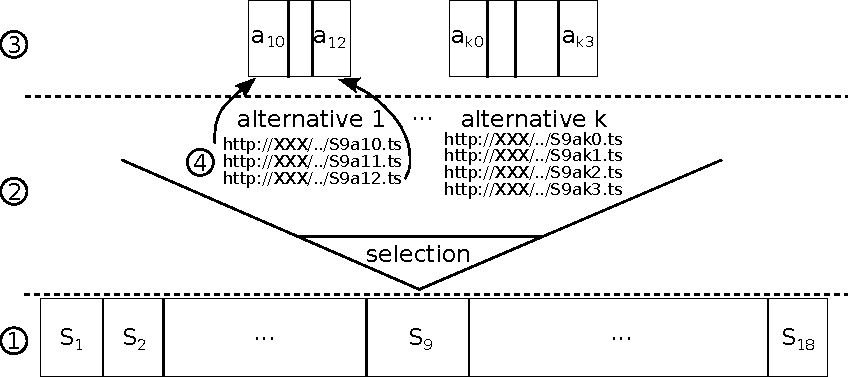
\includegraphics[width=1\linewidth]{figures/bref-generator.pdf}
\vspace*{-4mm}
\caption{\label{fig:generator}Video generator: modularity and variants}
% \vspace*{-4mm}
\end{figure}

Figure~\ref{fig:process} shows how the client and the server communicate to generate and play a video variant. First, the client asks for the generation of a new video. The server returns a list of file names corresponding to the selected sequences ($\{S1a2, ..., S18a4\}$ in our example).  
Each file corresponds to a playlist that defines the sub-parts of the sequence \eg in \ding{195} of Figure~\ref{fig:generator} the playlist defines 3 sub-videos: S9a10, S9a11 and S9a12.
The client downloads all the playlists and their corresponding videos. Finally, the client \emph{merges} the videos of the playlists and plays the resulting video variant.


\begin{figure}
\centering
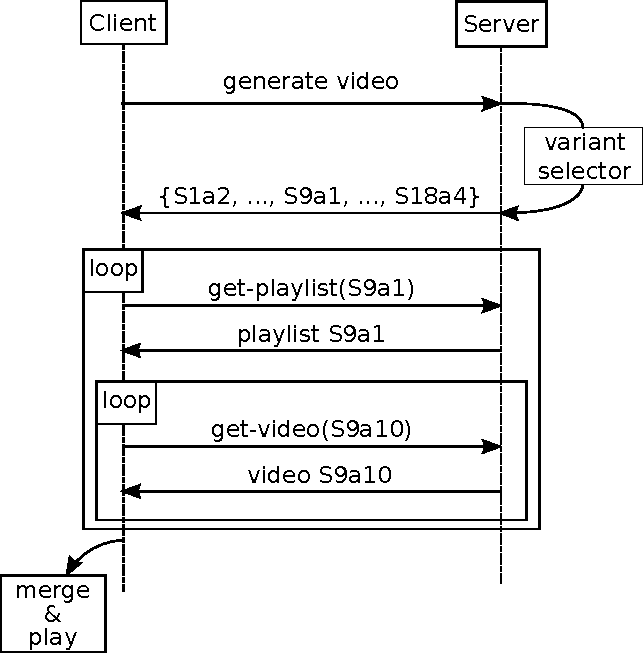
\includegraphics[width=0.7\linewidth]{figures/server-client.pdf}
\vspace*{-2mm}
\caption{\label{fig:process}Communications server/client}
\vspace*{-4mm}
\end{figure}





% We have then contacted the creators of the video generator with two research questions and goals in mind: (1) can we \emph{automate} the extraction of variation points and configurations (video variants)? (2) can we re-engineer another generator and configurator? 
% The creators accepted to collaborate and provided us with an access to an offline version of the generator. However we did not have access to the source code % neither in the server side nor in the client side. Like this, we can study the generator as a black box system -- as it would be the case in reality -- but without disturbing the deployed Web generator (e.g., with hundreds of HTTP requests). 
% \ma{We can remove this one: 
% The interest for the creators was to audit their systems.
 % security mechanisms for avoiding or at least complicating our tasks.
%




%  and defensive mechanisms have to be considered. 

\wprv
%
%  Our first audit showed that a reverse engineering work can get access to all the video sequences. Furthermore, ,
   % (see~\cite{BrefVamos14} for more details). 
% 15 new variation points are now apparent, out of which 13 are configurable (i.e., exhibiting at least 2 alternatives). 
% For the 3 variation points also present in the original configurator, users can now explicitly choose the alternatives. 
 The implementation of the product line can cause two important threats. 
The first threat is that an attacker can download the video sequences, which are protected by copyright. As digital content is a key business value, protecting the access to data becomes a security problem. Without defensive mechanisms, an attacker can extract and generate all the possible video variants of the original service. 
%
 The second consequence is that a new configurator can be re-engineered and could "kill the original idea"~\cite{BrefVamos14}. Specifically we showed it is straightforward to re-engineer a new generator and configurator in which users configure in a fine-grained way the 18 variations points -- instead of only 3 in the original version.
That is, with a re-engineered solution, the surprise effect is limited when getting a new video variant. Instead, users can control, choose and visualize \emph{any} alternative (video sequence). The creators of the generator did not have this intention  -- they did not want to jeopardize their trade secrets.

% calling to consider security issues. % -- though the idea of  
% -- thus dramatically limiting the \emph{surprise} effect. 

 % In other words, they have taken a strategic decision for, on-purpose, delimiting the scope of variability and restraining the visibility of some variation points and alternatives. 

% Our experience shows that the scoping of variability (i.e., what is visible to users) is a strategic solution and, 
% Overall the generator is well engineered and modularity is the right way to do from a development perspective. 
% Modularity is also needed to scale: as further emphasized in the next section, it is technically difficult to pre-generate millions of video variants.   \ma{says something like "modularity" or "featurization" is advocated by SPLE}

An important lesson learned is that the \emph{modularity} of data (video variants) poses a problem from a protection perspective.  
From a software engineering and product line perspective, modularity is undeniably good and remains a standing goal of any project. However modularity can backfire: an attacker can too easily understand the generation process and the differences between alternative sequences. 
With modularity, the task of determining the number of sequences and identifying the alternatives corresponding to each sequence does not face any obstacles. Similarly the collection and the \emph{composition} of video sequences is immediately understood. 
% Overall, a malicious attacker could not only collect all videos but could also launch a new competing video generator service; it is not acceptable.

Another important lesson learned is that an attacker should have difficulties to navigate into the configuration space. Otherwise she will be able to understand the whole product line and extract trade secrets in a \emph{comprehensive} and \emph{automatic} manner. Protection mechanisms for blocking frequent requests are worth considering but may not be sufficient. 
% An attacker can have difficulties to explore the modularity space.

 
% \ma{insist more on the "configurations" problem; rephrase or insist more on the "variability" aspect}




% \subsection{Windows Operating System Family}
% \label{sec:casestudy3}
% \dcs
%
 We describe some hacks related to the family of Windows operating systems. Microsoft sold its Windows products in three distinct packages: (1) \emph{full packaged product} is intended for installation on computers that have not previously had a licensed copy of the software; \emph{upgrade packages} offer a discount to owners of a previous edition of a given product; 
% In virtually all cases, the license terms require that you stop using the previous edition.
 (3) \emph{original equipment manufacturer} products offer the steepest discounts of all and are installed on new or refurbished computers.
% \end{itemize}

In 2008, an upgrade hack in Windows Vista allowed end users to purchase the upgrade edition and install it on any computer -- with no need to purchase the more expensive full edition. Interestingly, the upgrade disc contained in fact the \emph{whole} product line (\ie not just an upgrade).
%

In 2009, Windows 7 was subject to a hack that allows a clean install of the operating system using an upgrade disc rather than the full version upgrades~\cite{w7microsoft}. 
Eric Ligman, Microsoft senior sales excellence manager, wrote a series of blog posts. 
He recognized the hack but also warned users about licensing issues:
\begin{quote}
Over the past several days there have been various posts, etc. across a variety of social media engines stating that some "hack" shows that a Windows 7 Upgrade disc can perform a "clean" installation of Windows 7 on a blank drive from a technical perspective. 
Of course, from the posts I saw, they often forgot to mention a very basic, yet very important piece of information... "Technically possible" does not always mean legal. 
\end{quote} 
 % version 
% Some proprietary systems or applications hide on purpose some features. Users typically have to pay for activating the features. For example, 
% It calls for investigating \emph{variability-aware security} mechanisms. 

In 2014, Microsoft announced to stop supporting Windows XP, but a simple registry hack lets users continue to get security updates.
The registry setting makes Windows Update thinks Windows XP system is actually Windows XP POSReady (which is still supported). 
Hence a Windows XP machine can receive updates for another five years. %, without having to pay. 
Microsoft quickly reacted: 
\begin{quote}
% We recently became aware of a hack that purportedly aims to provide security updates to Windows XP customers. 
The security updates that could be installed are intended for Windows Embedded and Windows Server 2003 customers and do not fully protect Windows XP customers. Windows XP customers also run a significant risk of functionality issues with their machines if they install these updates, as they are not tested against Windows XP.
\end{quote}


\wprv
% 
 The stories with the different variants of Windows have some consequences. Users without a full license of Windows (e.g., Windows 7 Beta available during the trial phases) can fully install Windows 7. Users can apply continued security updates for Windows XP (despite the end of the support).
The naive implementation allows outsiders to easily modify the settings of the product line. The case shows that technical hacks may be employed to bypass Windows. Though all workarounds violate the terms of license agreements, Microsoft was forced to quickly react and communicate.  

 

\subsection{Web Configurators}
\label{sec:casestudy4}
\dcs
%
 % In many markets, organisations are competing to propose customised products, characterised by hundreds of inter-related \textit{configuration options}. 
 % As the repertoire of inter-related options can be disconcerting for many customers, \textit{Web configurators} are developed to assist them during decision making.
% As an example, Figure~\ref{fig:configurationDummy} shows a snapshot of a typical car configurator (the circled letters and legend can be ignored for now). 
 A Web configurator provides an interactive graphical user interface that guides the users through the configuration process, verifies constraints between options, propagates user decisions, and handles conflictual decisions~\cite{ebrahimCSMR2014}. %ebrahim2013}. %rogoll2004,streichsbier2009,Trentin2012}.
% Configurators are used in many applications to personalize products and services. 
 Configurators are used in installation wizards, preference managers, and extensively used in product lines. 
 %  
 The database maintained by Cyledge is a striking evidence with 900+ Web configurators coming from 30+ different industry sectors~\cite{configurators}. % ~\cite{configurators}
% \footnote{\url{http://www.configurator-database.com}}

% Since 2007, Cyledge collected more than 900 Web configurators coming from 30+ different industry sectors, including automotive, apparel, sport, and art. 
% 
 A very simple excerpt of a real-world Web configurator is depicted in the Figure below. % ~\ref{fig:configurationDummy}. 
We can observe that the selection of \textsf{Diesel} has lead to the automated selection of \textsf{EDC6}. (In fact, some other equipment options have been previously selected; one can select \textsf{Diesel} with \textsf{EDC7} or \textsf{BVM} in some other configuration settings.) 
That is, a customer has not chosen \textsf{EDC6}; the configurator has imposed some constraints of different natures: technical/engineering constraints, aesthetic constraints, marketing constraints, \etc


% \begin{figure}[!hts]
% \vspace*{-3mm}
% \begin{center}
% \includegraphics[scale=0.31]{img/configuratorDummy.png}
%   \vspace*{-7mm}
% \caption{Audi web SC (\texttt{http://configurator.audi.co.uk/}, Oct. 18, 2012)} %\url{
% \vspace*{-9mm}
% \label{fig:configurationDummy}
% \end{center}
% \end{figure}

\begin{figure}[!hts]
\centering
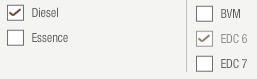
\includegraphics[scale=0.5]{figures/configuratorRenault.png}
% \vspace*{-2mm}
%\caption{{\small{Options and constraints in a configurator}}} 
% \label{fig:configurationDummy}
\vspace*{-2mm}
\end{figure}


% SCs represent a significant portion of the configurators used in modern information systems. %Their application domains range from y are used to automate the tuning of information systems to the preferences of the user. Installation wizards, preferences managers, and configurable business process models~\cite{quteprints12686,DBLP:conf/caise/GottschalkWJAR09} are examples thereof. 

% where multiple information system variants are derived from a base of reusable artefacts according to the specific characteristics of the targeted customer or market segment~\cite{Pohl2005,Schaler:2012:BIS:2363463.2363516,DBLP:conf/caise/GottschalkWJAR09,quteprints12686}. 

% A significant share of existing configurators is Web-based, irrespective of the market. 

% In this paper, we focus on web configurators supporting online sales.%, but we will argue that some of our findings generalize to other types of configurators.




% These configurators vary significantly. They each have their own characteristics, spanning visual
% aspects (GUI elements) to constraint management. 
% The web SC of Audi appearing in Figure~\ref{fig:configurationDummy} is thus only one example. It displays different options through specific widgets (radio buttons and check boxes -- \textcolor{red}{ \mycirc{A}} and \textcolor{red}{\mycirc{B}}, respectively). These options can be in different states such as activated (e.g., \configopt{Privacy glass} is flagged with \checkmark) or unavailable (e.g., \configopt{Twin-pane UV and heat-insulating glass} is greyed out). Additionally, these options are organised in different tabs (e.g., \configopt{Equipment}) and sub-tabs (e.g., \configopt{Equipment packages}) which denote a series of steps (\textcolor{red}{\mycirc{C}}) in the \emph{configuration process} (e.g., \configopt{1. Model} is followed by \configopt{2. Engine}-- \textcolor{red}{\mycirc{D}}). A SC can also implement \emph{cross-cutting\footnote{We call these constraints \emph{cross-cutting} because they are often orthogonal to the hierarchy of options, sub-options, etc. supported by the configurator.} constraints} between options (\textcolor{red}{\mycirc{E}}). These are usually hidden to the user but they determine valid combinations of options. For instance, the selection of \configopt{Privacy glass} implies the deselection of \configopt{Twin-pane UV and heat-insulating glass}, meaning that the user cannot select the latter if the former is selected. 
% Moreover, descriptive information (\textcolor{red}{\mycirc{F}}) is sometimes associated to an option (e.g., its price). % of the product.

\wprv
% As privileged channels for identifying customer needs and placing orders, configurators are key assets for companies. 
 Products, options, and the underlying constraints a configurator is in charge of are key information of an organization. 
Such information is particularly interesting from the perspective of (online) \emph{market intelligence (MI)} (also called \emph{competitive intelligence}). 
MI can be defined as the "information relevant to a company's
markets, gathered and analyzed specifically for the purpose of accurate and confident decision-making in determining
market opportunity, market penetration strategy, and market development metrics." 
Lixto, a company offering data extraction tools and services for MI, showed that it is technically feasible to acquire and exploit unstructured and semi-structured data in several case studies (\eg in the domain of computers and electronics consumer goods~\cite{baumgartner2009}). % 

Most information on pricing, product availability, product options, and product constraints is potentially available on Web sales configurators.
Specifically, competitors can use this information (1) for getting a comprehensive overview of the options and constraints in the market; (2) to be (continually) informed about strengths and weaknesses of other competitors' product lines; (3) to publicly reveal a certain superiority or marketing practice, \etc
  
 Web data extraction systems~\cite{baumgartner2009,Ferrara2014} can be specialized for acquiring configurators' information. 
 Early attempts~\cite{ebrahimCSMR2014} showed that reverse engineering Web configurators is feasible. Static analysis techniques can locate templates of options and some constraints in a Web page. % The major threat for companies developing Web configurators is that the templates followed 
  Combined with crawling techniques for deep navigation and dynamic content pages, there is the potential to comprehensively gather relevant information. 
%  Though 
  In case the static and dynamic analysis of variability can be seamlessly realized, there is a risk for companies developing Web configurators to reveal trade secrets. 
% and should provide 
 % Baumgartner \etal develop data extraction techniques and tools to improve the process of
% acquiring market information~\cite{baumgartner2009}. 
% A solid layer of knowledge is fundamental
% to optimize the decision-making activities and a large
% amount of public data could be retrieved on the Web. They to . 


% In particular, using the  Suite to access, extract, clean and deliver
% data, it is possible to gather, transform and obtain data useful
% to business purposes.

% Market intelligence comprises
% as a special case competitive intelligence. Online market
% intelligence (OMI) covers all aspects of MI that are related
% to online information sources, predominantly, to the
% Web. 





% \emph{B} 

% Analysing competitors' Websites. Web configurators coming from the same industry sector most likely present products with similar characteristics (e.g., configuration options). Using our proposed Web data extraction techniques, we can acquire market information from these competitors and compare their products (e.g., price comparison,
% option comparison). 




% Wider, the process of gathering and analyzing data about products,
% customers, competitors with the goal of helping the managers
% of a company in decisional processes is commonly called Competitive
% Intelligence, and is strictly related to data mining [58]. Zanasi
% [125] was the first to introduce the possibility of acquiring these
% data, through data mining processes, on public domain information.

% Chen et al. [22] developed a platform, that works more like
% a spider than a Web Data Extraction system, which represents a
% useful tool to support Competitive Intelligence operations. In Business
% Intelligence scenarios, we ask Web Data Extraction techniques
% to satisfy two main requirements: scalability and efficient planning
% strategies because we need to extract as much data as possible
% with the smallest amount of resources in time and space.




% Comparing prices; identifying a weakness;

% Users are forced to select some options (augmenting the price)
% Users have to follow a certain workflow 

% The Crawler can play a crucial role in exploring the configuration space and extracting dynamic data from different Web configurators (comprehensiveness) 



% \subsection{Other Cases}

% Our is by no means comprehensive.
% There are other product lines (and systems with variability) subject to protection issues. 
% We can cite the family of Windows operating systems (see the hacks with different variants of Windows 7~\cite{w7microsoft})
% The three case studies we discussed are not the only examples of product lines

% \section{Case Study 2}
% \label{sec:casestudy2}
% \subsection{\dcs}

\subsection{\wprv}

\subsection{\mechvar}

% \section{Case Study 3}
% \label{sec:casestudy3}
% \subsection{\dcs}

\subsection{\wprv}

\subsection{\mechvar}

% \section{Case Study 4}
% \label{sec:casestudy4}
% \subsection{\dcs}

\subsection{\wprv}

\subsection{\mechvar}

\section{Protect Variability!}
\label{sec:summary}
%\ma{Video games?}

%\begin{figure*}
%\begin{tabularx}{\textwidth}{|X|X|X|X|}
%\hline
%Case Study   & Description & Why protecting variability? & Protecting mechanisms \\ \hline
%Bref         &    an online video generator that plays humoristic video variants based on some users' choices and random choices &                       
%data protection (videos copyright); software protection (frequency distribution, access to data); discovery of variability may kill the "surprise" effect and kill the interest of the generator
% & demodularizing modularity; protections to limit the crawling of the configuration space             \\ \hline
% Newspapers   & online newspapers with four variants (for regular readers, members, journalists, web engine) & privilege access to content & everything in one place; feature interactions \\ \hline
%Windows 7    &     an operating system coming in different variants ("upgrades")       &  free upgrade                           & everything in one place                       \\ \hline
%%Automotive   &    embedded code in vehicles      &        may contain hidden features that can be activated                     &                       \\ \hline
%Configurator &    web configurators assist customers in selecting options and eventually choose a product &        marketing or technical constraints may be discovered; business intelligence;       &      protections to limit the static analysis of configuration options; to limit crawling of the configuration space                   \\ \hline
%\end{tabularx}
%\caption{Case studies}
%\end{figure*}
%
%\begin{itemize}
%\item barriers to crawling the configuration space 
%\item the danger of putting everything in one place
%\item obfuscation/demodularizing (code + data + mapping)
%\end{itemize}




% Previous section shows that possible vulnerabilities in the implementation of product lines can jeopardize trade secrets. 
We observe that the case studies are sharing similar classes of security and protection issues.
We identify three kinds of vulnerabilities (related to positive variability, negative variability, or configuration space) and leading to the possible leaks of trade secrets. 
We draw a research roadmap highlighting four directions (RD1, RD2, RD3, RD4).
% calling to investigate protection mechanisms.
% The overall challenge is to cross fertilize the research results in software product lines and security to efficiently protect variability.

% A tentative classification of these vulnerabilities can be done according to the use of either positive or negative variability. In this section, we classify the previous vulnerabilities according to these two use of variability, and we give some insights on how they would be consider to be protected according to the kind of variability implemented. In both cases,  
\rro{Protection of positive variability (RD1)} Voelter \etal describe variability implemented with \emph{compositional} approaches as positive variability since variable elements are added together~\cite{voelter2007}. 
It is the case of the video generator case study (see Section~\ref{sec:casestudy2}) in which video sequences are assembled to build a video variant. 
It may also be the case in Web configurators (see Section~\ref{sec:casestudy4}) in which options are added on-the-fly depending on some user choices. 

We have shown in Section~\ref{sec:casestudy2} that an attacker can too easily reverse engineer the product line with a clean modularization design. 
The vulnerabilities are coming from the identification of the modules and their direct mapping in terms of features in the variability model. From this identification, an attacker can infer how these modules can be composed together to re-engineer the product line (\ie by positive variability). 
It should be noted that the positive variability (and the underlying issues) apply either at the data level (e.g., videos) or at the implementation level (source code) of the product line. Two main approaches are then possible to prevent the discovery of trade secrets. 

First, source code deconstruction, such as control flow degeneration and data flow disturbance, are essential obfuscation techniques~\cite{collberg1997taxonomy}. 
% They can prevent reverse engineering and code tampering to protect intellectual property and business secrets. 
% Source code deconstruction, such as control flow degeneration and data flow disturbance, are essential techniques for code obfuscation. 
% For an overview on code obfuscation, we refer to the now classical taxonomy by Collberg and colleagues~.  
 An open challenge is to develop techniques for obfuscating specifically the variability and modularity in the source code or data.  
%
 A second approach is to obfuscate the \emph{mapping} between features/options and the corresponding artefacts. 
For instance, a one-to-one mapping may be too easy to identify and understand. 
The challenge is to develop innovative techniques, ideally non intrusive for product line developers and agnostic to a domain, for diversifying the mapping. 
 %  of the modules in terms of feature in the variability model \todos{here give more from the previous paper}. 
The two approaches can be used independently or in combination, depending on the product line characteristics. % of the product line.

% The first category consists in obfuscating the source code and the data. 

% \emph{Data obfuscation} aims at obscuring the purpose of the artefacts and the data structures that a program manipulates during its execution~\cite{naumovich2003preventing}.
% In~\cite{collberg1998breaking} several techniques are proposed to demodularize Java classes and data types by breaking their structures. In particular, they propose to split % or merge arrays. We can relate this example to our case study as we also propose to split or merge sequences of videos.
% The main difference with our work is the nature of the data. In our case, we consider the demodularization of external artefacts such as video files instead on focusing on the internal variables and data structures of a program.


%Why is obfuscation a kind of diversification?
% A basic obfuscation technique simply transforms a program $P$ in a program $P'$ which is distributed. 
 % Since obfuscation is automated, it is often possible to generate several different obfuscated versions of the same program (as proposed by Collberg \etal~\cite{collberg12} for example).
% Wang \etal \cite{wang01} propose a multi-level program transformation that aims at degenerating  the control flow so as to provide in-depth obfuscation. %This work on program transformation takes place in the context of a software architecture for survivable systems as proposed by Knight et al. \cite{knight00}. 
% Wang's approach consists in two main steps: transform all high-level control flow structures in \emph{if-then-goto} structures; introduce aliases in the goto statements so that the goto address is determined only at runtime.
%In both cases, this kind of technique results in a semantic diversity of execution profiles, and consequently is deeply related to automated diversity.
%  Another approach consists in letting programs self-modify. These programs embed a runtime randomization technique \cite{mavrogiannopoulos2011taxonomy}, which will modify the binary code in way that attackers cannot retrieve the structure of the control or data flow. This is done for sake of security and is considered one of the strongest obfuscation mechanism~\cite{mavrogiannopoulos2011taxonomy}. 
%
 
 
 
% security purposes to (1) external data operated by a program (e.g., as needs be in our case study); (2) adapt or generate the code in charge of accessing de-modularized data. 

% ~\cite{DBLP:series/ais/Rinard11}
% 
% ~\cite{DBLP:conf/aosd/Rinard12}

% \subsection{}
% Altering the source code initially developed, either at compile or at runtime, is a common approach that was already investigated for other non functional properties than security (e.g., performance).
% For example, in the context of quality of service, 
 % Sidiroglou \etal~\cite{Sidiroglou-Douskos2011} have introduced loop perforation and shown that in some domains it is possible to skip the execution of loop iterations. 
% For instance, in a video decoding algorithm (codec), skipping some loop iterations has an effect on some pixels or contours but does not further degrade or crash the software application. On the other hand, skipping loop iterations is key with respect to performance. 
% In other words, it is possible to manipulate a program's functionality to handle performance or  security issues~\cite{Rinard11}. This trade-off can be set offline (e.g. by arbitrarily skipping one every two loops) or dynamically based on the current load of the machine or intrusion detection.

% This approach is also intensively used in the context of optimizing compilers that try to optimize some properties in the generated code (e.g., execution time or memory consumption). Such approaches that act at compile time apply some static analysis of the source code, and adapt the design for optimization purpose. For example, the polyhedral model \cite{quillere2000} is commonly used for loop nest optimization to detect where a set of loop transformations can be applied for the purpose of locality optimization or parallelization.

% Besides, numerous techniques have been proposed to automate the remodularization of an existing software project~\cite{DuBois2004,Bryton2008,Zanetti2014,Goldstein2014}. The goal is rather to improve modularity properties, for instance, to ease the maintenance of an application. 

% All exposed techniques in this section offer \emph{demodularizing} mechanisms. Some of them have different goals and do not necessarily target security issues. We believe some of these techniques could be applied for our class of problem. 


% The challenge is to develop 
% and are complementary. 
 

%, e.g., decomposition into module \todos{here give more from the previous paper}. 




% once and for all
% at once
% straightaway
% right from the beginning
\rro{Protection of negative variability (RD2)} Some product lines exhibit all their functionality and content once and for all. They use \emph{negative} variability (as opposed to the previous positive variability) in which all different variants are expressed; the variants are activated depending on some conditions. 
It is the case of online newspapers (see Section~\ref{sec:casestudy1}). 
%  and the Windows family (see Section~\ref{sec:casestudy3}). 
 It may also be the case in Web configurators (see Section~\ref{sec:casestudy4}) in which options are hidden or depicted on-the-fly depending on some user choices. The source code of such configurators already contains the content for activating/deactivating options typically through JavaScript. 
% Web configurators (see Section~\ref{sec:casestudy4}) in which options are added on-the-fly depending on some user choices. 
% Scenarios Z and ZZ have shown vulnerabilities in the particular configuration of a given product. In this case, the initial product provide all the features which are restricted according to the expected features (aka. negative variability). 
 Negative variability cannot be accused of being the root cause of vulnerabilities. However, it is necessary to either:
\emph{(1)} improve the mechanism used to remove or activate some variants. For instance, access controls (e.g., at the server side) or obfuscations can be considered; \emph{(2)} obfuscate the pre-defined variants. For example, in the case of online newspapers, the content of members' articles can be encrypted.
% \end{itemize}
% To prevent the identification of the possible configurations, 

% \todos{here give more from the previous paper}. 

An interesting research direction is to determine whether (and if yes, when) negative variability presents more security guarantees than positive variability (or the other way around). Product lines can indeed use the two kinds of variability (\eg as in Web configurators). 

\rro{Barriers to master the configuration space (RD3)} Understanding a configuration set may have an interest \emph{per se} since trade secrets are hidden there. 
For example, the video generator of Section~\ref{sec:casestudy2} has a strategy for generating some frequencies of features. The idea is that some features corresponding to some video sequences are rarely activated (e.g., in 0.1\% of configuration) for surprising the visitor. 
As another example, Web configurators exhibit options with marketing or technical constraints. 
In the two examples, the ability of an attacker to crawl the configuration space is the key for discovering trade secrets. The more, better it is. A \emph{comprehensive} visit is the worst situation since the extracted knowledge is then complete. %
 Another threat of a (comprehensive) mastering of the configuration space is that attacker can experiment the effects the configurations have on the product line. 
It is one of the basis to understand or guess the underlying implementation of a product line.
% For example, setting specific configuration settings in the registry of Windows (see Section~\ref{sec:casestudy3}) proves to give access to some features of the product line. 
 In the video generator, setting a configuration leads to a new video variant that can be then analyzed. 
A comprehensive visit is again the worst situation since all corresponding variants and related artefacts are then accessible.

%  a configuration set may have 

% In the two aforementioned categories, discovering the modularization or removal mechanism of the features leads to the identification of the set of configurations that this mechanism can support. However, this does not allow an attacker to identify the particular constraints between certain features, preventing certain undesirable configurations. Such constraints can be discovered by 
The challenge of RD3 is to develop barriers to limit the exploration of the configuration space. 
For instance, some mechanisms for blocking temporarily internet protocol addresses can be considered in case many requests for crawling the configuration space are observed (see Section~\ref{sec:casestudy2}). Many specific factors can influence the definition of a politics of configuration access. % limiting accesses is specific to a product line since




% systematically exploring the set of configurations on the system (or by using more sophisticated algorithm to limit the exploration space). To address this issue, it is necessary to prevent the systematic exploration of the configurations, depending on the intended use of the product line. 

% For example ...

\rro{RD4: Cost-benefit tradeoffs} On the one hand, protecting variability and configurations has admittedly a cost. 
The technical or management effort can be more or less important -- from a drastic change in the design of the product line to small increments to re-enforce access controls. 
On the other hand, the trade secrets an organization has to protect and the possible consequences highly vary. A trade secret can give access to very few non-members, but can also lead to lose any competing advantage. 

Hence a tradeoff has to be found. The importance of trade secrets a product line can jeopardize should justify the investments required to develop and deploy protecting mechanisms. A spectrum of more or less sophisticated techniques can thus emerge. 
% An expected quality (and challenge) is to have 
 An ideal solution (hence a challenge) is to let product line developers follow their usual methods while guaranteeing adequate security. % configurations
 
% of deriving the individual products during application engineering

% to the lose of millions of customers 



%\subsection{\mechvar}
%
%% 
%
%We now discuss some defensive protection strategies in the context of our case study. 
%In particular, as modularity is exposing security threats, we define and describe possible \emph{demodularization} mechanisms, i.e., disruptive mechanisms capable of adapting the original modularity.
%
%\subsubsection{Basic Protection}
%
%\ma{emphasize that protection is to (1) limit "configuration crawling" (2) obfuscate the "code" (not the data) so that we can have difficulties to understand the variability implementation}
%
%Numerous protections exist against reverse engineering or illegal access, in particular in the domain of Web applications as in our case study.
%For instance, it is possible to forbid suspicious connections and block temporarily some internet protocol addresses. 
%An attacker can have difficulties to explore the modularity space. 
%
%Another basic strategy is to obfuscate client code (JavaScript) to make the attacker's tasks harder. 
%A first obstacle is that obfuscation may have some limits and debuggers can partially reduce the desired effect. Another severe limitation -- the most important one -- is that the behaviour logic is also visible through communication traces (HTTP requests) with the server. 
%% More generally obfuscation 
%% not only expressed at the JavaScript 
% 
%Actually, these two protections were enabled in our case study. But an attacker is still able to reverse engineer the service and get access to the videos. 
%In fact, these techniques try to hinder a possible reverse engineering but do not hide all forms of modularity present in other artefacts (e.g., video playlist).
%This motivates the need for techniques that hide or transform the original modularity of data and code as perceived by an attacker.
%
%\subsubsection{Demodularization and Heartbreaking} 
%
%\ma{we have to reduce}
%
%A first technique would be to remove all or part of the modularity in a video.
%In our example, it would result in \emph{merging} all the video sequences on the server side. 
%That is, a video variant would then consist in one and unique sequence instead of 18. 
%
%With such demodularization strategy, there is no need for playlists and video sequences. 
%A benefit is that the attacker has only access to a full, monolithic video variant at a time; the modularity units are no longer present, complicating the reverse engineering process. %task  
%% This heavily complicates the task of an attacker.
% Let say, in this context, an attacker still wants to understand what are the alternatives for each portion of the video. He or she would have to download numerous video variants, and then find commonalities and differences between portions of the videos. The difference of two or more than two videos is not an easy task, requiring to rely on image processing algorithms. A manual review is also needed to specify when and how the video sequences should be cut (the length of alternatives varies). 
% 
% % especially in the case study where alternatives significantly differ. 
%
%% and finally detect the sequences.
%Though appealing, the idea of merging video sequences has significant drawbacks. The operation should be realized in the server side for assembling video sequences. It is resource and time-consuming, precluding a reactive, scalable service. A more subtle strategy would be \emph{pre-}generate and store the video variants before a client's request. Generating all the video variants is not feasible as it represents billions of videos. 
%This technique also significantly increases the needs for computation power and storage of the hosting infrastructure.
%
%Overall the demodularization strategy exposed in this subsection has severe drawbacks since all good properties of modularization are lost. 
%
%\subsubsection{Varying Variability Through Demodularization Strategies}
%% Demodularizing Strategies} 
%%\section{}
%
%\ma{we have to reduce}
%
%Other strategies can be considered to adapt the modularity of the video generator so that an attacker either (1) perceives differently and wrongly the original modularity or (2) has severe difficulties to recover and understand the original modularity.  
%
%
%For instance a disruptive technique is to artificially increase the modularity. For example, the server can (randomly):
%\begin{itemize}
%\item add empty videos to the playlist;
%\item change the order of the videos;
%\item modify file names associated to video sequences.
%\end{itemize}
%
%% is it more like shifting modularity?
%
%Another technique is to change the modularity structure. For example, the cutting of video sequences can vary. 
%% be implemented differently -- conceptually stay at 18 
% Instead of observing 18 video sequences, an attacker would observe, say, 9 sequences. 
%This time, 9 playlists associated to the 9 sequences would actually be constituted of two playlists of successive alternatives.  
%More sophisticated combinations can be envisioned as well while the cutting can be randomly shifted for each client. As a result, an attacker would see a different structure at each request. But internally and eventually the video variants would still be assembled as 18 video sequences. 
%The benefit is that an attacker will have severe difficulties to identify and locate the modularity units, because of a random modification of the modularity structure. 
% 
% % It would hinder the access to all the videos and thus the re-engineering of a new service.
%
%Overall, breaking the modularity of the original service can increase its security as it highly disrupts the comprehension of modularity by attackers. 
%However, we note that breaking the modularity at design time may directly impact the development of the application. That is, more engineering effort may be needed to realize an efficient demodularization technique. In some cases, the demodularization involves the modification of different artefacts (e.g., JavaScript source code, generation of video playlists) in the server side and the client side.
%% This may even lead to go against fundamental guidelines of software engineering. % cancel the benefits of building a modular application and 
%
% Therefore, the focus should be put on generative techniques that act later in the lifetime of an application (\eg at compile or run time). This would allow to keep good properties of modularity when developing and still have a more secured application. %  with respect to modularity.



% \section{Related Work}
% \label{sec:related}
% %\bb{Obfuscation}
%\bc{Two areas of work: (1) breaking some artefact for improving other non functional property eg performance (M. Reiner) (2) demodularization strategies}

% \subsection{Code obfuscation}
Software is composed of two elements: code and data~\cite{WirthAlgorithms}.
Demodularizing source code has been extensively studied, as we show in the following. However, only a few works have focused on \emph{demodularizing the external data and the source code in charge of accessing data}. 

\emph{Data obfuscation} aims at obscuring the purpose of the artefacts and the data structures that a program manipulates during its execution~\cite{naumovich2003preventing}.
In~\cite{collberg1998breaking} several techniques are proposed to demodularize Java classes and data types by breaking their structures. In particular, they propose to split or merge arrays. We can relate this example to our case study as we also propose to split or merge sequences of videos.
The main difference with our work is the nature of the data. In our case, we consider the demodularization of external artefacts such as video files instead on focusing on the internal variables and data structures of a program.

Source code deconstruction, such as control flow degeneration and data flow disturbance, are essential techniques for \emph{code obfuscation}. Code obfuscation aims at preventing reverse engineering and code tampering to protect intellectual property and business secrets.
%Why is obfuscation a kind of diversification?
% A basic obfuscation technique simply transforms a program $P$ in a program $P'$ which is distributed. 
 Since obfuscation is automated, it is often possible to generate several different obfuscated versions of the same program (as proposed by Collberg \etal~\cite{collberg12} for example).

Wang \etal \cite{wang01} propose a multi-level program transformation that aims at degenerating  the control flow so as to provide in-depth obfuscation. %This work on program transformation takes place in the context of a software architecture for survivable systems as proposed by Knight et al. \cite{knight00}. 
Wang's approach consists in two main steps: transform all high-level control flow structures in \emph{if-then-goto} structures; introduce aliases in the goto statements so that the goto address is determined only at runtime.


%In both cases, this kind of technique results in a semantic diversity of execution profiles, and consequently is deeply related to automated diversity.

Another approach consists in letting programs self-modify. These programs embed a runtime randomization technique \cite{mavrogiannopoulos2011taxonomy}, which will modify the binary code in way that attackers cannot retrieve the structure of the control or data flow. This is done for sake of security and is considered one of the strongest obfuscation mechanism~\cite{mavrogiannopoulos2011taxonomy}. 
%
 For an overview on code obfuscation, we refer to the now classical taxonomy by Collberg and colleagues~\cite{collberg1997taxonomy}.  

% ~\cite{DBLP:series/ais/Rinard11}
% 
% ~\cite{DBLP:conf/aosd/Rinard12}

% \subsection{}
Altering the source code initially developed, either at compile or at runtime, is a common approach that was already investigated for other non functional properties than security (e.g., performance).
% For example, in the context of quality of service, 
 Sidiroglou \etal~\cite{Sidiroglou-Douskos2011} have introduced loop perforation and shown that in some domains it is possible to skip the execution of loop iterations. 
For instance, in a video decoding algorithm (codec), skipping some loop iterations has an effect on some pixels or contours but does not further degrade or crash the software application. On the other hand, skipping loop iterations is key with respect to performance. 
In other words, it is possible to manipulate a program's functionality to handle performance or  security issues~\cite{Rinard11}. This trade-off can be set offline (e.g. by arbitrarily skipping one every two loops) or dynamically based on the current load of the machine or intrusion detection.

% This approach is also intensively used in the context of optimizing compilers that try to optimize some properties in the generated code (e.g., execution time or memory consumption). Such approaches that act at compile time apply some static analysis of the source code, and adapt the design for optimization purpose. For example, the polyhedral model \cite{quillere2000} is commonly used for loop nest optimization to detect where a set of loop transformations can be applied for the purpose of locality optimization or parallelization.

% Besides, numerous techniques have been proposed to automate the remodularization of an existing software project~\cite{DuBois2004,Bryton2008,Zanetti2014,Goldstein2014}. The goal is rather to improve modularity properties, for instance, to ease the maintenance of an application. 

% All exposed techniques in this section offer \emph{demodularizing} mechanisms. Some of them have different goals and do not necessarily target security issues. We believe some of these techniques could be applied for our class of problem. 


% The challenge is to develop 
% and are complementary. 

The challenge is to apply demodularization strategies for security purposes to (1) external data operated by a program (e.g., as needs be in our case study); (2) adapt or generate the code in charge of accessing de-modularized data.  




% software based on move refactoring, i.e. moving classes
% between packages without changing any other aspect of the source
% code.

% \ma{It should be noted that some approaches advocate modularity for realizing security (out of the scope, but funny to notice)}


\textbf{Concluding remarks.}
\label{sec:conclusion}
In this paper, we provided evidence that product lines can jeopardize their trade secrets. 
% Other product lines (\eg in the domain of video games~\cite{videogames}) are certainly subject 
 % Our vision is that it is urgent to cross-fertilize the research results in software product lines and security. 
% The trend to exhibit product lines on the Web certainly explains why the problem has not been considered so far.
 % 
 Any software systems may come up against security/protection issues, yet the specificities of handling variability/configurations raise novel and difficult challenges. 
 % We identified several research directions for protecting the internal software variability and configurations of product lines.
We mainly took the perspective of a defender; the research can be considered from an attacker point of view as well (though ethics and legal aspects have to be defined). 
% The major challenge is to determine when the trade secrets of a product line outweigh investments required to develop and deploy adequate protecting mechanisms. 
 For concluding, we formulate the idea that software variability of product lines, as a key competing advantage and first-class citizen, should itself vary to complicate the task of an external attacker. % suggest?

%  considered 
%  Exhibiting a product line comes with some threats

 % to efficiently protect product lines.



\textbf{Acknowledgements.} We thank anonymous reviewers for their valuable feedbacks.
%
% The following two commands are all you need in the
% initial runs of your .tex file to
% produce the bibliography for the citations in your paper.
\scriptsize
%\vspace*{-2mm}
\vspace*{-1.4216431810035168mm}
\bibliographystyle{abbrv}
\bibliography{DEModularity15}  % sigproc.bib is the name of the Bibliography in this case
% You must have a proper ".bib" file
%  and remember to run:
% latex bibtex latex latex
% to resolve all references
%
% ACM needs 'a single self-contained file'!
%
%\balancecolumns

% That's all folks!
\end{document}
